\section{SeafloorAI}
{{\footnotesize
\begin{description}[labelwidth=5em, labelsep=1em, leftmargin=*, align=left, itemsep=0.3em, parsep=0em]
  \item[date:] 2024-12-13
  \item[version:] TODO
  \item[last\_updated:] 2024-12
  \item[expired:] unknown
  \item[valid:] yes
  \item[valid\_date:] TODO
  \item[url:] \href{https://neurips.cc/virtual/2024/poster/97432}{https://neurips.cc/virtual/2024/poster/97432}
  \item[doi:] TODO
  \item[domain:] Marine Science; Vision-Language
  \item[focus:] Large-scale vision-language dataset for seafloor mapping and geological classification
  \item[keywords:]
    - sonar imagery
    - vision-language
    - seafloor mapping
    - segmentation
    - QA
  \item[summary:] A first-of-its-kind dataset covering 17,300 sq.km of seafloor with 696K sonar images, 827K segmentation masks, and 696K natural-language descriptions plus \textasciitilde{}7M QA pairs-designed for both vision and language-based ML models in marine science :contentReference[oaicite:1]\{index=1\}.

  \item[licensing:] TODO
  \item[task\_types:]
    - Image segmentation
    - Vision-language QA
  \item[ai\_capability\_measured:]
    - Geospatial understanding
    - multimodal reasoning
  \item[metrics:]
    - Segmentation pixel accuracy
    - QA accuracy
  \item[models:]
    - SegFormer
    - ViLT-style multimodal models
  \item[ml\_motif:]
    - Vision-Language
  \item[type:] Dataset
  \item[ml\_task:]
    - Segmentation, QA
  \item[solutions:] TODO
  \item[notes:] Data processing code publicly available, covering five geological layers; curated with marine scientists :contentReference[oaicite:2]\{index=2\}.

  \item[contact.name:] Kien X. Nguyen
  \item[contact.email:] unknown
  \item[datasets.links.name:] Sonar imagery + annotations
  \item[datasets.links.url:] \href{\textasciitilde{}15 TB}{\textasciitilde{}15 TB}
  \item[results.links.name:] ChatGPT LLM
  \item[fair.reproducible:] Yes
  \item[fair.benchmark\_ready:] Yes
  \item[ratings.software.rating:] 0
  \item[ratings.software.reason:] Not analyzed.

  \item[ratings.specification.rating:] 9.0
  \item[ratings.specification.reason:] Real-time qubit classification task clearly defined in quantum instrumentation context.

  \item[ratings.dataset.rating:] 9.0
  \item[ratings.dataset.reason:] Dataset available on Zenodo with signal traces; compact and reproducible.

  \item[ratings.metrics.rating:] 9.0
  \item[ratings.metrics.reason:] Accuracy and latency are well defined and crucial in this setting.

  \item[ratings.reference\_solution.rating:] 9.0
  \item[ratings.reference\_solution.reason:] GitHub repo has reproducible code and HLS firmware targeting FPGA.

  \item[ratings.documentation.rating:] 8.0
  \item[ratings.documentation.reason:] Good setup instructions, but no interactive visualization or starter notebook.

  \item[id:] seafloorai
  \item[Citations:] \cite{nguyen2024seafloor}
  \item[Ratings:]
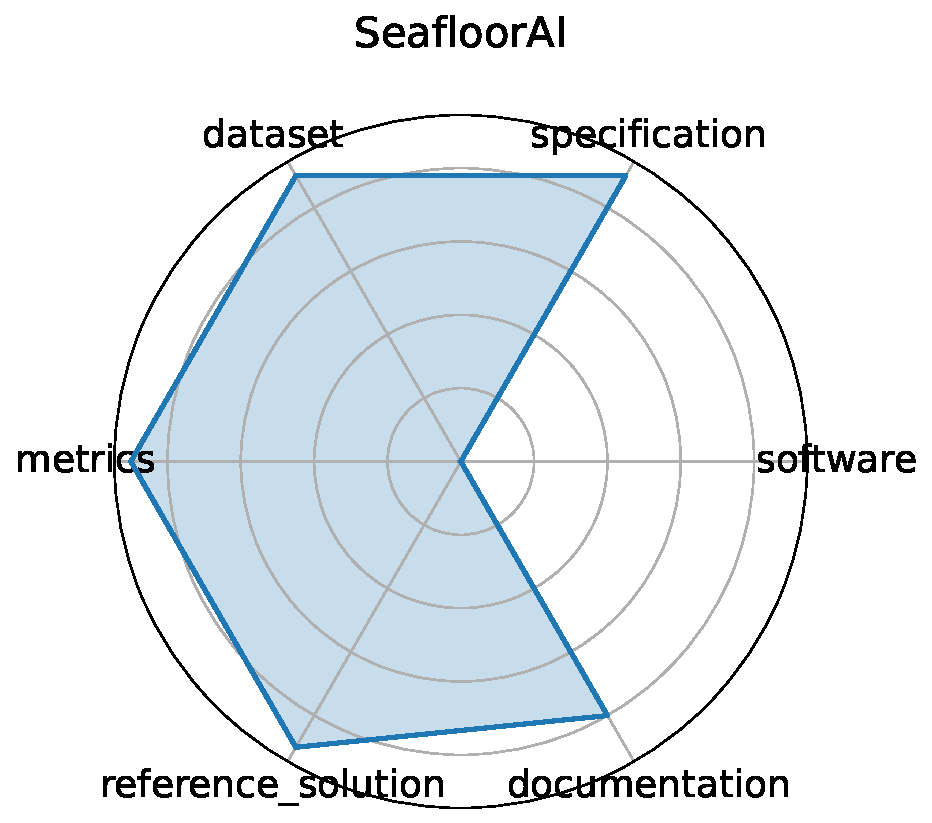
\includegraphics[width=0.2\textwidth]{seafloorai_radar.pdf}
\end{description}
}}
\clearpage